% !TeX root = ../../thesis.tex
\chapter{Materials and methods}
\label{ch:methodology}

% \section{Genomic sequence data}
%
% For both Hepatitis B and Lassa analyses our genomic sequence came from a variety of sources.
% Both analyses were comprised of a majority of sequences pulled directly from publically available sequence databses.
% Additionally, both analyses include a subset of novel sequences generated by their respective study groups that have not yet been released publically.

\section{Bayesian phylogeographic inference of HBV}

\subsection{Genomic sequence data}
We analyze a total of 1,590 complete Hepatitis B virus genomes divided among three genotypes, and arising from three primary sources: publically availabe sequence databases, novel genomes sequenced by collaborators, and recently sequenced ``ancient'' genomes isolated from mummies.
The genomes that we analyze were divided into three datasets based on their HBV genotype, such that we had 587 HBV-A genomes, 769 HBV-D genomes, and 234 HBV-E genomes.
Of these, the vast majority (total 1,466: 540 HBV-A, 765 HBV-D, 170 HBV-E) were provided by collaborators following a query of the GenBank sequence database. %GB: this begs the question where the other ones came from; you can mention this information and prepare for questions (rudimentary ones) on how these data were generated, i.e. which technology (Illumina, MinION, ...).
In order to investigate temporal signal in these HBV data sets, we perform additional analyses by including---for two genotypes---recently published ``ancient'' genomes isolated from mummies ranging in age from 450 years old to 4,500 years old \cite{muhlemann2018ancient, ross2018paradox}. %GB: I would make sure to mention `ancient' as this will tie in nicely with your explanation of measurably evolving populations in the introduction, where you should talk about `ancient DNA' data sets and mention Beth Shapiro's Science paper on bison populations.
The underlying assumption is that these genomes may help to improve temporal signal in the HBV datasets, as typically remarkably little signal is present in such data.
We will assess whether the addition of these ancient samples allows to infer approximate timing windows of historical events.

\subsection{Preprocessing}

Prior to Bayesian inference, we estimated unrooted maximum likelihood phylogenetic trees using IQ-TREE\cite{nguyen2015iq}.
These maximum likelihood trees were used to perform temporal signal analysis using TempEST\cite{rambaut2016exploring}---a tool which quantifies temporal signal by performing regression analysis of genetic divergence over time---allowing us to remove sequences that showed incongruent temporal signal patterns.
%GB: The next two sequences are technically results.
The resulting dataset comprised 583 sequences of HBV-A genotype viruses, 764 HBV-D sequences, and 234 sequences HBV-E genotype viruses.
With the inclusion of ancient genomes, the final HBV-A and HBV-D datasets included 587 and 769 total taxa, respectively.

\subsection{Phylogenetic modeling}

We inferred phylogenetic trees for each of our three datasets by performing Bayesian inference using MCMC as implemented in \gls{beast}1.10\cite{suchard2018bayesian}.
For all datasets we used the same model specification as detailed below.
Branch rates were inferred under an uncorrelated relaxed molecular clock model assuming an underlying lognormal distribution, allowing us accommodate evolutionary rate variation across the branches of the phylogeny.
Following unsuccessful modeling of demographic history under a Bayesian skygrid model, we used a constant demographic model as a tree model. %GB: I don't mind this sentence, but it can lead to questions
%BP: I wasn't sure how to nicely tie the non-results into the thesis, so I was planning on making it part of the presentation.
To accommodate the impact of the overlapping regions in the HBV genome on the substitution process of each codon position, we assumed an HKY substitution model\cite{hasegawa1985dating} without codon partitioning, accommodating among-site rate heterogeneity through a discretized gamma distribution\cite{yang1993maximum}.
We performed at least three independent replicates of our \gls{mcmc} analysis to ensure proper convergence, with each replicate running for 500 million iterations and subsampling every 10,000th iteration. %GB: make sure to be specific as to which approaches help with convergence and which help with mixing, as these are entirely different aspects
We assumed default priors in \gls{beast} for all parameters these analyses except for lognormal substitution rate with mean $\mu=-11.3474$ and standard deviation $\sigma^{2}=1.22)$, %GB: I would avoid this type of math notation (it's also not defined what X is) and simply write down the mean and standard deviation (and mention the correct scale)
which was derived from the HBV substitution rate estimated by the researchers who generated the ancient genomes \cite{muhlemann2018ancient}.
To speed up likelihood computations we used the BEAGLE 3 high-performance computational library.
MCMC chains were run for 500 million iterations and were sampled every 25,000th state.
For each subtype, multiple replicates were run in parallel using different starting seeds to ensure proper convergence and statistical mixing, and a single combined posterior distribution was formed from all replicates, removing an appropriate proportion (at least 10\%) of each chain as burn-in.
From this combined posterior distribution, 1,000 trees were sampled and used to perform subsequent Bayesian phylogeographic reconstruction in \gls{beast} using empirical tree distributions.
We perform phylogeographic inference on an empirical tree distribution because joint inference of both discrete geographic history and phylogenetic history was found to be computationally intractable.

\subsection{Phylogeographic modeling}

\newglossaryentry{mcc}{name={MCC},description={Maximum clade credibility}}
\newglossaryentry{ctmc}{name={CTMC},description={Continuous-time Markov chain}}
\newglossaryentry{bssvs}{name={BSSVS},description={Bayesian stochastic serach variable selection}}
\newglossaryentry{bf}{name={BF},description={Bayes factor}}
Employing the collected empirical tree distributions, we estimated the spatial diffusion dynamics using a Bayesian phylogeographic approach in which the locations are treated as discrete traits, and allowed for different migration rates to and from each location.
This approach conditioned on the geographic locations recorded at the tips of the trees and models the transition history among those locations as a continuous-time Markov chain (\gls{ctmc}) process to infer the unobserved locations at the internal nodes of each tree.
For these reconstructions, \gls{mcmc} chains were run for 10 million iterations and sampled every 10,000th state.
Maximum clade credibility (\gls{mcc}) trees were summarized using TreeAnnotator v1.10 (cite \gls{beast} 1.10) and the resulting trees were visualized in FigTree v1.4.3.
The links between locations that contribute significantly to explaining the migration history were identified using a Bayesian stochastic search variable selection (\gls{bssvs}) procedure, and SpreaD3\cite{bielejec2016spread3} was used to calculate the Bayes factor (\gls{bf}) support for these links.
We also estimated the expected number of location state transitions in the ancestral history conditional on the data observed at the tree tips using ``Markov jump'' counts, providing a quantitative measure of asymmetry in viral flow between regions.
Since the data consist of a heterogeneous number of sequences for each location which show strong sampling bias between individual countries that can strongly impact the outcome of a discrete phylogeography study.
To mitigate this issue, we opted to group sequences into pseudo-continental regions, aiming to contain a number of sequences of the same order of magnitude where possible: Africa, the Americas, East \& South Asia, Europe, and West \& Central Asia, which created a more even split than country or continent-level divisions.
We note that for data set E, no samples from East \& South Asia, nor West \& Central Asia were available.

\section{Lassa phylogenetics and online inference}

\subsection{Genomic sequence data}

In recent years the cost of generating genomic sequence data has dropped substantially\cite{sboner2011real}.
This, coupled with improvements to the speed and usability of software packages for analyzing these data, has led to an explosion of genomic sequence availability in recent years.
With high-throughput molecular sequencing, genomic data from pathogenic viruses are becoming available in unprecedented quantities and with remarkable speed, even in resource-limited settings, aided by portable genome sequencing technology.
One such example was during the 2013--2016 West African Ebola outbreak, during which a novel sequencing protocol was developed and implemented to perform an unprecedented number of genomes from the oubread ``in the field'' in real-time\cite{quick2016}.
The end result of this was a steady flow of new genomes during the course of the epidemic, resulting in roughly 5\% of all cases producing a genome\cite{dudas2017virus}.
As such technologies continue to be refined, constant generation of genomes in real-time will become increasingly common during viral outbreaks\cite{jain2016oxford}.
For the ``new'' \gls{lasv}genomes that we analyze as a part of this thesis, we use data generated using one such mobile sequence platform---the Oxford Nanopore MinION.
Though our data is generated using this particular techonology, the automated build pipeline that we introduce in the following sections is not dependent upon sequencing technology.

\subsection{Preprocessing and model specification}

Beyond the runtime complexity of currently available phylogeographic inference tools real time analyses are further impeded by the significant amount of preprocessing that they necessitate before raw sequence data can be analyzed.
This preprocessing generally takes the form of bespoke pipelines that require significant manual work to function properly.
While each individual analysis presents challenges unique to the biology of the pathogen of interest, for many analyses the general scheme of data preprocessing is similar.

The prototypical preprocessing pipeline begins with collection of genomic sequence data.
It is not uncommon for genomic data to come from multiple disparate sources.
Genomic databases (e.g. GISAID\cite{shu2017gisaid}, ViPR\cite{pickett2012vipr}, GenBank\cite{benson2012genbank}) frequently present data to the user in a variety of formats---presenting a major hurdle towards systematically collating genomes into a single dataset.
Additionally, researchers performing analyses frequently wish to include genomes generated by their own research groups or collaborators.
These genomes will generally not be stored on database servers, preventing them from being available to database APIs that could normally assist in the building of datasets.

Even after full datasets are assembled, they may not be the final set of sequences that will be used for phylogenetic inference.
Frequently, researchers wish to downsample their datasets based on a variety of factors---both assisting with runtime and reducing the risk of introducing sampling bias into the final analyses.
Specific genomes may be deemed inappropriate for analysis based on containing incomplete or highly ambiguous sequences.
Genomes may also be excluded based on genetic distance thresholds or their phylogenetic placement in previous analyses.
In addition to removing specific inappropriate sequences, researchers will frequently downsample randomly (or pseudorandomly) to achieve a desired distribution of genomes through time, space, or some other feature of interest.
Finally, researchers may want to ensure that specific sequences are included in their analyses for a variety of reasons, and thus ensure that they are not removed by downsampling procedures.
When running online analyses, it is often desired that the updated set of new sequences need to be included in the analysis, requiring them to be exempt from downsampling.

Following the generation of a suitable dataset of genomes, there are are still several necessary steps that must take place prior to phylogenetic inference that generally require significant manual work.
An important prerequisite step for all molecular phylogenetic inference is the generation of a multiple sequence alignment of all the input genomes.
Many different alignment tools are available to perform this task (e.g. BWA, MUSCLE, MAFFT), however they are generally highly parameterized tools with many available options that must be explored to create a suitable alignment.
This step in particular often requires a large amount of manual work; many parameter combinations must be explored and alignments must be inspected manually as they cannot be easily validated automatically.
Addition of new sequences in an online setting---though programatically simple if there is an existing framework---must still be validated manually in most cases, posing an obstacle to fully automated build pipelines.

Once an alignment has been generated, phylogenetic models must be specified; this is often a very complicated task.
Some models can be specified in \gls{beast} using its graphical interface, BEAUti.
Unfortunately this program does not support the full suite of models that \gls{beast} can run at this time, and its use in facilitating online phylogenetic analyses is even more limited.
Indeed, for many features that researchers may wish to use the only method for specifying them is by editing code blocks in a source file manually.
While this process is possible to automate for those with sufficient technical knowledge there is no existing method for first-time users of the \gls{beast} ecosystem to do so.
In addition to initial model specification, it is frequently the case that models need to be tweaked follow some runtime either to be optimized or to fix issues that occur during their execution.
This process is currently performed entirely manually by the user, further impeding automatic phylogenetic analysis.

The final preprocessing step necessary before Bayesian phylogenetic analysis can be performed is the specification of \gls{mcmc} parameters.
This step generally takes place in concert with model specification, as its exact details vary significantly with different statistical models.
Chain length---the number of iterations that the program will run---scales non-linearly with dataset size, dataset complexity, and model complexity; it is often estimated as a best guess by the user and cannot be explicitly calculated.
It is often the case that a particular \gls{mcmc} chain length is either insufficient to adequately explore the posterior distribution of all parameters, or it is vastly larger than necessary, resulting in excess computational resource being devoted to an analysis.
Prior distributions for all parameters must be specified prior to analysis, and may need to be updated significantly following the addition of new data in an online setting.
Similarly, operators that modify each parameter during a run are particular to each model parameter and may change dynamically as data is introduced to an online build.
Indeed, operators may also need to be changed if they are found to not work well for a given dataset---some may operate too ``slowly'' and not explore state space adequately, while others may lack the power to deviate from local extrema in state space and become ``stuck'' for thousands, if not millions, of states.
Only after all of these steps have been completed can a user begin to perform the actual phylogenetic inference that interests them.

\subsection{Adaptable bipartite build framework}

Lassa virus (LASV) proves to be a particularly difficult virus to preprocess for the purposes of phylogenetic inference.
In particular, generating an accurate and useful alignment can be very challenging with LASV due to its high sequence variability.
The challenges from this variability are compounded, as they need to be accounted for both across Lassa's two genomic segments, but also for the two genes on each of the segments, which need to be aligned to each other to provide meaningful results during phylogenetic analysis.
To handle these challenges, we divide our adaptable processing framework into two steps, one for alignment generation, and one for build parameterization and specification.

\subsubsection{Snakemake for build management}

For both of these steps, we employ the use of Snakemake \cite{koster2012snakemake}, a flexible workflow management system designed to be used with the Python programming language, to manage build specifications and easily perform online Bayesian inference.
We use this as an alternative to the traditional methods of workflow management---most commonly simple shell scripts or repeated use of command line tools.
The use of Snakemake in our build pipelines affords us three major advantages over previous methods of build management: increased build reproducibility, easy parameterization, and robust error management.

A pipeline is broken into its component steps as a series of ``rules''---each encapsulating a single command line directive---that can be parameterized by a single configuration file.
Each rule is defined in terms of its expected input and output as filenames; each rule also specifies a particular directive that should generate the outputs from the input.
For example, one could specify a rule, \texttt{count\_lines}, whose goal was to apply the \texttt{wc -l} command line utility to an \texttt{input.txt} file and generate an \texttt{output.txt} file.
At runtime Snakemake would check that \texttt{output.txt} did not already exist on the filesystem---an important check that prevents costly recomputation.
Next, Snakemake would check if \texttt{input.txt} existed on the filesystem, yielding an error if the file were not present.
Snakemake would then apply the specified command line utility.
Finally, Snakemake would check that \texttt{output.txt} existed in the filesystem, throwing an error if the expected file were not present.
Importantly, Snakemake allows us to generalize these steps so that one's input is determined as a function of the previous step's output, and to apply dynamic changes to the workflow according to user specified variables.
This combination of rules strung together, plus filesystem checks to determine presence or absence of input and output files, affords us the opportunity to update builds quickly and without performing unnecessary recomputations.

Because each command is centralized into the Snakemake workflow, exact reproduction of past analyses becomes trivial.
Indeed, reproduction of past analyses with minor alterations (e.g. a slightly updated dataset, different \gls{mcmc} chain length) also becomes trivial, as all parameters are saved in a single configuration JSON file, rather than memorized or stored in shell history.
This is of particular importance because it allows for easy specification of updated builds without running the risk of losing previously performed analyses due to filesystem overwrites (a concern when using shell scripting or command line copy/pasting).
It also ensures that all build parameters and commands that are not explicitly modified by the user are kept constant, ensuring consistency between builds.

\subsubsection{Alignment generation}

Our initial Lassa analyses began with genomes gathered from GenBank via API query and from previously unpublished genomes from 2019 seasonal outbreaks in Nigeria provided by collaborators (671 L segments, 795 S segments)\cite{kafetzopoulou2019metagenomic}.
Midway through the analysis period we received incoming data updates from collaborators in Nigeria, increasing our dataset sizes to respectively 698 L segments and 826 S segments.
Data from collaborators were provided to us as Microsoft Excel spreadsheets containing both sequences and metadata, necessitating a preprocessing pipeline that could collate new genomes with those generated by GenBank query.
For each sequence, its genotype was determined according to BLAST\cite{boratyn2013blast} search.
Genotype-gene alignments were then built using MAFFT and concatenated ``vertically'' across genotypes\cite{katoh2013mafft}.
Finally, alignments were concatenated ``horizontally'' between the two genes for each segment, padded with \textit{N} characters to allow for variations in length and to buffer between genes.
This process is illustrated in Figure~\ref{fig:alignment_dag}.

\newglossaryentry{dag}{name={DAG},description={Directed acyclic graph}}
\begin{figure}[ht]
  \centering
  \medskip
  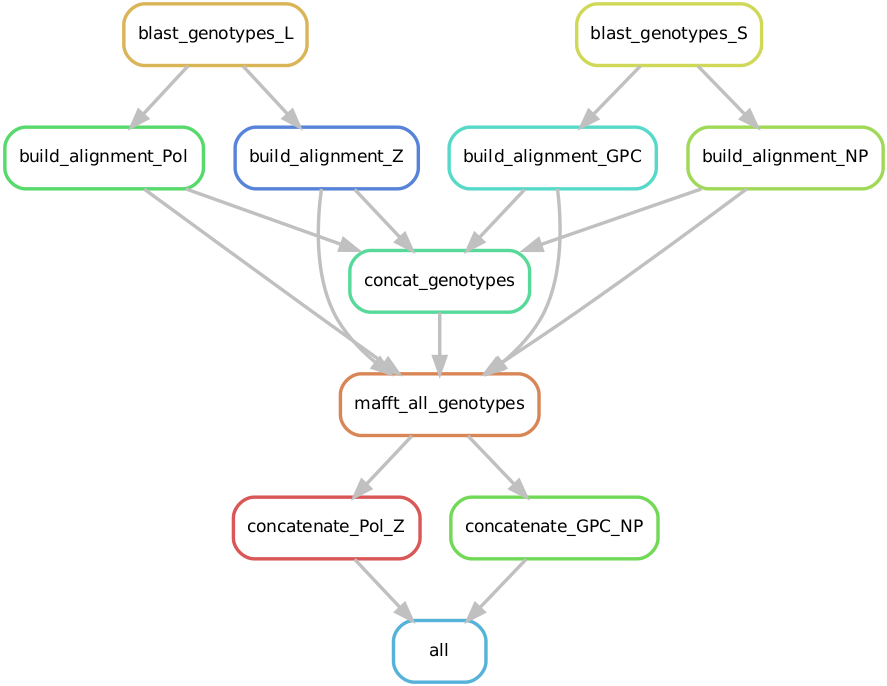
\includegraphics[width=.9\textwidth]{alignment_dag}
  \caption[Lassa alignment pipeline]{A directed acyclic graph (\gls{dag}) representing the pipeline by which we generate Lassa virus alignments. We first use BLAST on each segment to determine its genotype. We then build gene-specific alignments for each genotype, and concatenate the results ``vertically''---i.e. all alignment files are combined into one. Then, we update the alignments such that all genotypes are as well aligned with each other as possible. Finally, we combine each gene ``horizontally'' within each segment---i.e. for each segment and each strain there is a single sequence in the alignment---such that the final result are two final alignment files, one for each genome.}
  \label{fig:alignment_dag}
\end{figure}

\subsubsection{MCMC build specification}

\newglossaryentry{hmc}{name={HMC},description={Hamiltonian Monte Carlo}}
For our Lassa analyses, we created a Snakemake pipeline similar in form to that used for preprocessing.
This pipeline (Fig.~\ref{fig:workflow_dag}) took the output alignments described above as its primary input.
From each, we generated \gls{beast} XML files.
We use a Bayesian skygrid demographic models for our analyses---though the pipeline is parameterized to easily accommodate both constant population size and Bayesian Skyride demographic models.
Our Skygrid inference used a Hamiltonian Monte Carlo (\gls{hmc}) operator to allow efficient transition of population size state space\cite{baele2020hamiltonian}.
We assumed an HKY substitution model with codon partitioning for each gene, accommodating among-site rate heterogeneity through a discretized gamma distribution.
We otherwise assume default \gls{beast} values for operators and priors.
The \gls{mcmc} chain length, logging frequency, and number of parallel replicates were parameterized dynamically though Snakemake, however for the results we present we ran a single chain for $5\times10^7$ iterations, logging every 15,000th state.

For each segment, after its parallel \gls{beast} replicates were completed, we remove burn-in from each log (minimum 10\%), and concatenate logs to form one joint posterior sample set.
We perform an identical process for posterior trees.
We use these combined parameter and tree distributions to generate MCC trees for each segment.

\begin{figure}[ht]
  \centering
  \medskip
  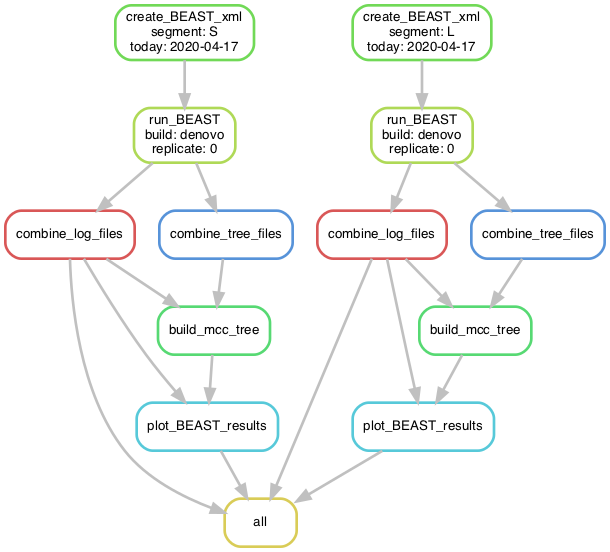
\includegraphics[width=.9\textwidth]{workflow_dag}
  \caption[Lassa phylogenetics pipeline]{A directed acyclic graph (DAG) representing the pipeline by which we perform Lassa virus phylogenetic inference. We perform identical workflows for each genomic segment. After \gls{beast} XMLs are generated and run, we remove burn-in and analyze the results of combined parameter and tree distributions.}
  \label{fig:workflow_dag}
\end{figure}

%%%%%%%%%%%%%%%%%%%%%%%%%%%%%%%%%%%%%%%%%%%%%%%%%%
% Keep the following \cleardoublepage at the end of this file,
% otherwise \includeonly includes empty pages.
\cleardoublepage

% vim: tw=70 nocindent expandtab foldmethod=marker foldmarker={{{}{,}{}}}
